
The project contains multiple containers, each built from scratch. Each container has its purpose. 
To create all the images for the containers there is a script, 0\_build\_images.sh, that will build 
all the images for the containers. 
The start\_terminals.sh script will take the argument to spawn n \acp{uav}. 
This will start multiple containers and it gives the user a terminal tab for each container. 
The code in each container is in a catkin package. Catkin is the official build system of \acs{ros}. 

\begin{figure}[ht]
    \centering
    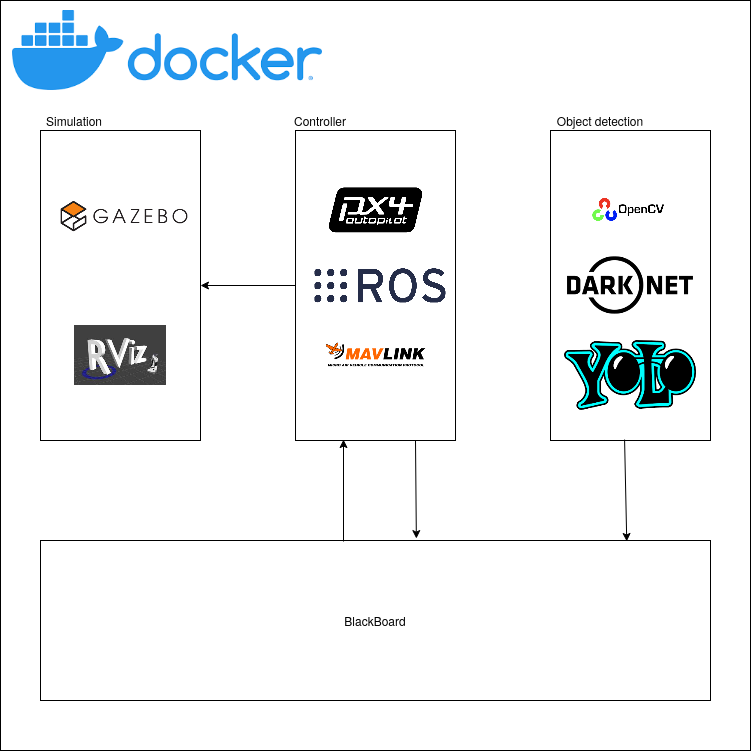
\includegraphics[scale=0.45]{dockerscheme.png}
    \caption[dockerscheme]{dockerscheme\footnotemark.}
\end{figure}

The first container is responsible for running Gazebo, the simulation. 
The container is built with the image \textit{smart\_uav\_px4} 
from another project built by fellow colleagues Vic Segers and Borcherd Van Brakel. \acs{ros}, MAVLink, 
MAVROS, PX4 firmware are all installed on this image. 
The simulation container is responsible for spawning all the \acp{uav} in a world. As previously, 
the script \textit{generate\_launch.sh} creates a launch file 
by generating a string and then writing this string to the \textit{smartuavs.launch} file. 

Inside this launch file a xarco file is passed as an argument for each \acs{uav}. 
The xarco file, \textit{iris\_base.xarco}, that is passed is in the folder \textit{rotors\_description/urdf}. 
The file takes two arguments, a \acs{tcp} and a \acs{udp} port. Giving each \acs{uav} different \acs{udp} and 
\acs{tcp} ports gives the ability to control each \acs{uav} separately. 

Inside the \textit{iris\_base.xarco} file all the components for the iris \acs{uav} are added. 
Before adding a component the file where it is originated must be included first. 


\begin{verbatim}
    <xacro:include filename="$(arg rotors_description_dir)
                                /urdf/component_snippets.xacro" />

\end{verbatim}

After including the xarco file, a component can be added to the \acs{uav}. 
Some components can take arguments like the \acs{3d} camera, the \textit{vi\_sensor\_depth\_macro}, 
can take some arguments on where to place the camera, how to orient the camera, 
a namespace, a parent link, a camera suffix (for the topic where it publishes its data to) and a framerate. 

\begin{verbatim}
    <xacro:vi_sensor_depth_macro
        namespace="${namespace}"
        parent_link="base_link"
        camera_suffix="iris_depth"
        frame_rate="30.0">
    <origin xyz="0 0 0.01" rpy="0 1.57079632679 0"/>
    </xacro:vi_sensor_depth_macro>

\end{verbatim}

If there is only one \acs{uav}, \acs{sdf} files can be used to simplify the process. The reason xarco files are used \acs{uav} is that 
they can take arguments 
whereas \acs{sdf} files can not. 
This means the \acs{udp} and \acs{tcp} ports can not be adjusted so only one \acs{uav} can be controlled \cite{sim:issue}. 

\newpage
The simulation container also contains Rviz, a \acs{3d} simulation tool for \acs{ros}. A developer can add topics, 
for example a point cloud from the camera, 
and Rviz will visualize this data.     
Finally to run the simulation and Rviz there is a script called \textit{1\_run\_launch.sh} inside the container. 
As a first argument (-a) it takes n amount of \acp{uav}. The default value is the n amount of \acp{uav} previously 
iven by starting the containers. 
The second argument (-w) is a path to a world file. The third argument (-g) is a boolean if Gazebo needs to have a visualization window. 
Without a window for gazebo the performance is a lot higher because of the limitation in gazebo rendering all 
the data, thus giving a better real-time factor.

\begin{figure}[ht]
    \centering
    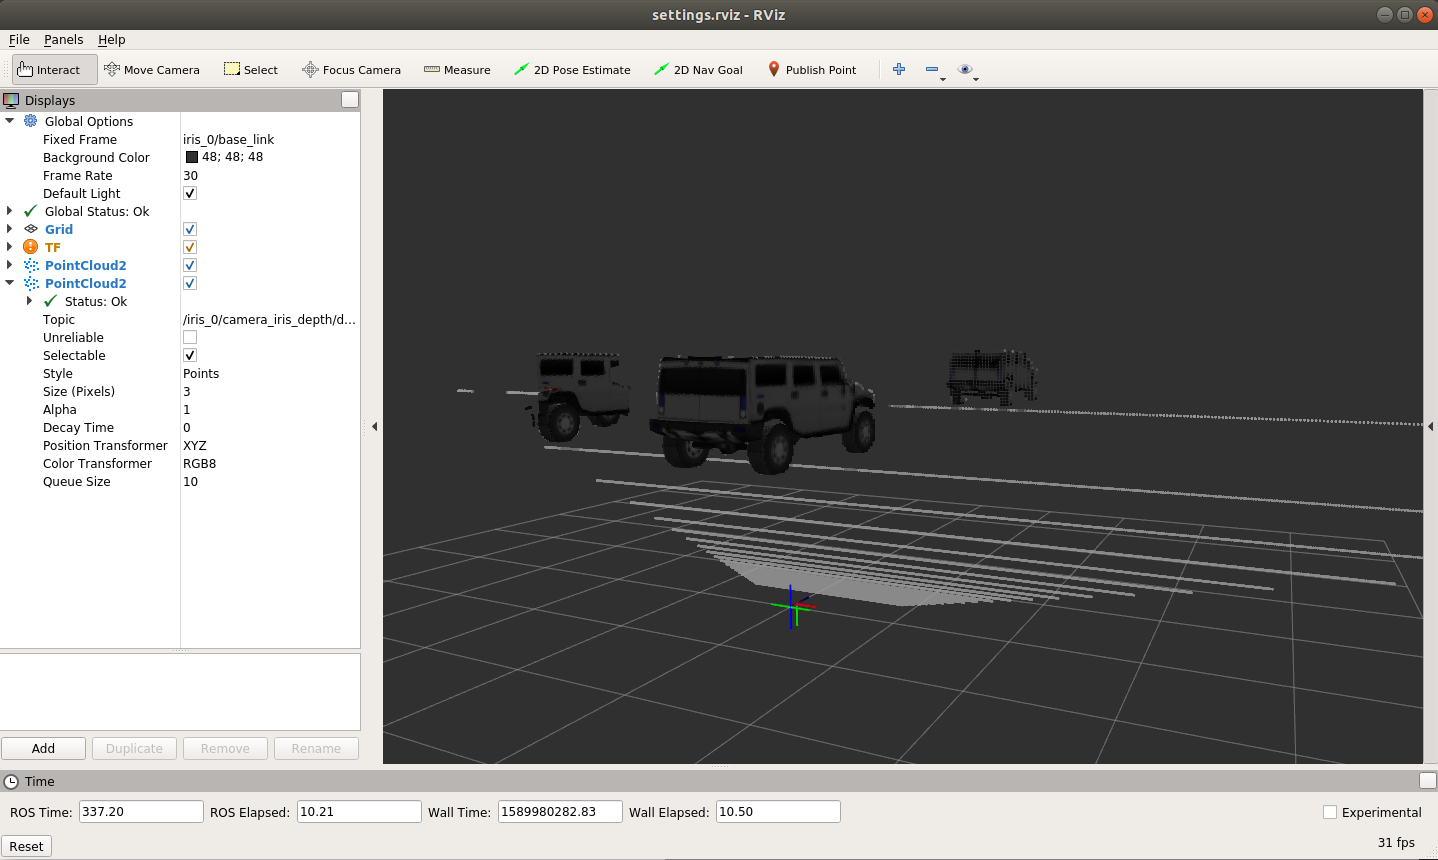
\includegraphics[scale=0.2]{RVIZ.png}
    \caption[RIVZ]{RVIZ\footnotemark.}
\end{figure}

Rviz, abbreviation for \acs{ros} visualization, is a visualization software that allows a developer to view data from Gazebo (or real-world). 
It can capture data, capture sensor information, replay captured data and provide a viewpoint of a robot. All this information 
comes in the form of topics. 
A developer can choose multiple topics in Rviz to visualize. Rviz has the ability to visualize multiple topics at the same 
time while maintaining high performance. 
By viewing the standpoint from a robot debugging is made substantially easier for a developer \cite{ros:rviz}.


Logging information is a crucial part of developing with \acs{ros}. Rosbags provide an easy way of logging information. 
These files can be quite large so \acs{ros} provided a way of capturing only crucial data. 
One or more topics can be listed after the command “rosbag record”, capturing only data given by the user. When playing back this rosbag will 
loop over the data, while Rviz visualizes it. A developer can use this for tracking down bugs, optimizing code, implementing features, etc.